\subsection{题目描述}
\noindent One-dimensional Kronig-Penney problem. Considering the Hamiltonian of the system as 
\[
\hat{H} = -\frac{\hbar^2}{2 m_e} \frac{\partial^2}{\partial x^2} + V(x)
\]
with a one-dimensional periodic potential \( V(x) = V(x + a) \). The potential can be expressed as 
\[
V(x) = 
\begin{cases}
0, & \text{if } 0  \leq x < L_W, \\
U_0, & \text{if } L_W \leq x < a
\end{cases}
\]
and the period of the potential is $a = L_W+L_B$, which is also shown in the Figure below.

\begin{figure}[H]
    \centering
    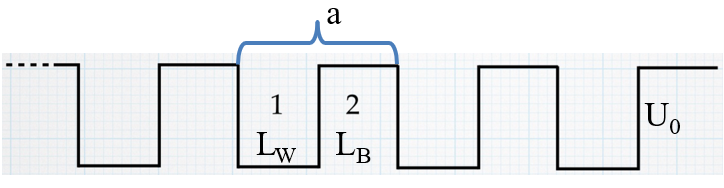
\includegraphics[width=1.0\textwidth]{Problem_1/figs/potential_well.png}
    \caption{Kronig-Penney potential well}
\end{figure}
\noindent With parameters:
\[
U_0 = 2 \, \text{eV}, \quad L_W = 0.9 \, \text{nm}, \quad L_B = 0.1 \, \text{nm} \quad (a = 1 \, \text{nm})
\]
Using FFT, find the lowest three eigenvalues of the electric eigenstates that satisfy 
\[
\hat{H} \psi_i = E \psi_i \quad \text{and} \quad \psi_i(x) = \psi_i(x + a).
\]
Explanation: Since the system is translation-invariant, i.e., \( \psi_i(x) = \psi_i(x + a) \), we can use the plane wave basis expansion 
$$ \psi(x) = \frac{1}{\sqrt{a}} \sum_q C_q e^{i q \frac{2\pi}{a} x} ,\quad q = -N, -N + 1, \dots, -1, 0, 1, \dots, N - 1, N .$$

\noindent In this basis set, the Hamiltonian can be represented in matrix form as
\[H_{pq}=\frac{1}{a}\langle e^{ip\frac{2\pi}{a}x}|\hat{H}|e^{iq\frac{2\pi}{a}x}\rangle_{\mathrm{cell}}=\frac{1}{a}\int_{0}^{a}dx e^{-ip\frac{2\pi}{a}x}\hat{H}e^{iq\frac{2\pi}{a}x}.\]
To calculate \( \hat{H} e^{i q \frac{2\pi}{a} x} \), the periodic potential \( V(x) \) can be expanded in Fourier series as \( V(x) \rightarrow V_q \), where 
\[ V(x) = \sum_{q'=-N}^{N} V_{q'} e^{i q' \frac{2\pi}{a} x} .\]
The basis wave function can then be written as:
\[\hat{H}e^{iq\frac{2\pi}{a}x}=(\hat{T}+\hat{V})e^{iq\frac{2\pi}{a}x}=\frac{2\hbar^2q^2\pi^2}{m_e a^2}e^{iq\frac{2\pi}{a}x}+\sum_{q^{\prime}=-N}^NV_{q^{\prime}}e^{i(q^{\prime}+q)\frac{2\pi}{a}x}\]
Try constructing the Hamiltonian matrix \( H_{pq} \) and solve the eigenvalue equation \( \hat{H} \psi_i = E \psi_i \) to obtain the three lowest energy eigenvalues.

\noindent \textit{Special note:} You can use built-in functions to simplify the eigenvalue calculations and FFT transformations.


\subsection{程序描述}
\textit{这道题的过程和结果都太神奇了。}

我们先顺着题目未完成的思路进行下来,计算哈密顿矩阵元
\[
H_{pq} = \frac{1}{a}\left\langle e^{ip\frac{2\pi}{a}x} \left| \hat{T} \right| e^{iq\frac{2\pi}{a}x} \right\rangle + \frac{1}{a}\left\langle e^{ip\frac{2\pi}{a}x} \left| \hat{V} \right| e^{iq\frac{2\pi}{a}x} \right\rangle
\]
其中动能项是对角阵
\[
    \frac{1}{a}\left\langle e^{ip\frac{2\pi}{a}x} \left| \hat{T} \right| e^{iq\frac{2\pi}{a}x} \right\rangle = \frac{\hbar^2}{2 m_e} \left( \frac{2\pi q}{a} \right)^2 \cdot\frac{1}{a}\int_0^a e^{-ip\frac{2\pi}{a}x} e^{iq\frac{2\pi}{a}x} dx= \frac{\hbar^2}{2 m_e} \left( \frac{2\pi q}{a} \right)^2 \delta_{pq} = \frac{2 \hbar^2 \pi^2 q^2}{m_e a^2} \delta_{pq}
\]
利用
\[
\left\langle e^{ip\frac{2\pi}{a}x} \left| e^{iq'\frac{2\pi}{a}x} \right| e^{iq\frac{2\pi}{a}x} \right\rangle = \int_0^a e^{-ip\frac{2\pi}{a}x} e^{iq'\frac{2\pi}{a}x} e^{iq\frac{2\pi}{a}x} dx = \int_0^a e^{i(q' + q - p)\frac{2\pi}{a}x} dx = a \delta_{p - q, q'}
\]
可以发现,势能矩阵元很自然地承载势能的傅里叶系数
\[
    \frac{1}{a}\left\langle e^{ip\frac{2\pi}{a}x} \left| V(x) \right| e^{iq\frac{2\pi}{a}x} \right\rangle = \sum_{q'=-N}^N V_{q'} \cdot \frac{1}{a} \left\langle e^{ip\frac{2\pi}{a}x} \left| e^{iq'\frac{2\pi}{a}x} \right| e^{iq\frac{2\pi}{a}x} \right\rangle=\sum_{q'=-N}^N V_{q'} \delta_{p - q, q'} = V_{p - q}
\]
注意到我们对实数域的势能展开时$V_{-q^{\prime}}=V_{-q^{\prime}}^{*}$,所以最后的哈密顿矩阵是厄米阵。


不过这里有个小漏洞,原本$p - q$的取值应该在$[-2N,2N]$,但我们在傅里叶展开势能为$V_{q^\prime}$的时候只展开到了$q^\prime \in [-N,N]$,所以按题意需要将 $p - q$ 截断在$ p - q  \in [-N,N]$ 之间(在赋值的时候加一组布尔掩码),这样才能保证$\sum_{q'=-N}^N V_{q'} \delta_{p - q, q'} = V_{p - q}.$

我原本认为这样是不合理的,应该将势能展开到$q^\prime \in [-2N,2N]$,而不是选择牺牲势能项的精度。但在助教提示下发现,本题的势能项本身影响就不大,所以这样的截断是可以接受的。在主程序中我也对这一点进行了对比论证,详见结果示例。

在最初阅读题干时,我最不明白的是,如此简单的阶梯函数已经可以解析计算出势能的傅里叶展开
\[
V_{q^{\prime}}=\begin{cases}\frac{U_0L_B}{a},&q=0\\\frac{U_0}{i{q^{\prime}}2\pi}\left(e^{-i{q^{\prime}}2\pi\frac{L_W}{a}}-1\right),&q\neq0\end{cases}
\]
随后想到这节课毕竟是在学习FFT,故在主程序中加入了FFT变换(实空间离散化再传递给\texttt{scipy.fft})的系数与解析计算的系数进行对比,发现两者差异在容许范围内,后面的计算则是基于解析计算的系数进行的。

源代码在\texttt{src/KP\_well.py}中,请在该目录下运行\ccmd{python -u KP\_well.py}即可得到结果,需要安装\texttt{numpy}与\texttt{scipy}库辅助运算,\texttt{matplotlib}库绘图。结果非常神奇,在大规模的绘制与计算中,我们发现了疑似二重简并的现象。在与QM1荣誉课的助教老师讨论后,合理怀疑是有限$N$的截断带来的边界效应,且在高能级时非局域化更明显,两侧的对称传播似乎是合理的。可惜在\texttt{debug}时我尝试过绘制其它相邻能级的波函数概率分布,未发现明显对称性。二重简并的原因有待进一步探讨,但能级的$n^2$增长是可以确认的。

\noindent \boxed{\textit{补充}}在与助教老师讨论后理解了,二重简并源自晶格势能的劈裂。原本的自由粒子动能项在有限基组中展开会能级离散化,随后不对称(原点没平移好)的势能诱导了正负动量的对称破缺,引发近似二重简并现象,且第一个能级应该对应原本的零动量态。感谢辛老师!

\noindent \boxed{\textit{补充}}与冯爹讨论之后推翻之前的结论,平移势阱为偶函数后仍会有第一个非零值,为势能的平均效应,且两侧能级的间隙未消除,详见\texttt{src/KP\_well\_even.py}.

\subsection*{主程序流程描述}

1. \textbf{初始化物理常量与参数}:从\texttt{const}获取需要使用的物理常数(如 $\hbar$、$m_e$ 等),定义参数,如 $U_0$、$L_w$ 和 $L_b$。
   
2. \textbf{傅里叶系数计算对比}:均采用自然顺序$[0,1,2,\dots,N,-N,\dots,-1]$,便于切片负数索引
   \begin{itemize}
       \item 使用\texttt{compute\_Vq\_analytical}方法计算势能傅里叶系数,基于解析表达式,
       \item 使用\texttt{compute\_Vq\_fft}方法,通过FFT计算傅里叶系数,验证解析方法的精确性。
       \item 比较两种方法的结果,输出最大和平均差异。
   \end{itemize}
   
3. \textbf{小规模收敛性检查}:借助\texttt{check\_convergence}函数,在较小 $N$ 下进行能级收敛性测试。

4. \textbf{AB方法对比}:
   \begin{itemize}
       \item \textbf{方法A}:在傅里叶系数范围 $Vq' \in [-N, N]$ 下进行求解,得到小规模能级,
       \item \textbf{方法B}:在扩展傅里叶系数范围 $Vq' \in [-2N, 2N]$ 下进行求解,
       \item 比较两种方法的能级差异,在之后计算中遵循题意采用方法A.
   \end{itemize}

5. \textbf{中等规模$N=100$计算与绘制}:
   \begin{itemize}
       \item 使用解析方法计算的傅里叶系数,构建哈密顿量矩阵,通过\texttt{solve\_eigenvalues}方法得到能级和波函数,
       \item 使用\texttt{reconstruct\_wavefunction\_vectorized}重构波函数,充分考虑基底正交性,归一化操作不需要积分,
       \item 通过\texttt{plot\_wavefunctions\_and\_potential}绘制势阱和前三个波函数,
       \item 绘制能级图,发现在小规模$N$中未出现的二级简并现象。
   \end{itemize}

6. \textbf{大规模计算与拟合}(可选):在用户确认的情况下
\begin{itemize}
\item  使用更大 $N=500$ 计算较多能级,
\item 通过\texttt{curve\_fit}函数拟合能级间距与量子数的平方增长关系,
\item 输出拟合系数并绘制拟合结果。
\end{itemize}

\subsection{伪代码}
Powered by \href{https://chatgpt.com/g/g-xJJAA2awf-latex-pseudocode-generator}{\LaTeX \ pseudocode generator}

\begin{algorithm}[H]
    \KwIn{$U_0$, $L_w$, $L_b$, $N_{initial}$, $num\_levels_{initial}$, $medium\_N$, $medium\_num\_levels$, $large\_N$, $large\_num\_levels$}
    \KwOut{Energy levels and wave functions, potential well plots, convergence analysis}
    
    \SetKwFunction{CompareFourierMethods}{compare\_fourier\_methods}
    \SetKwFunction{CheckConvergence}{check\_convergence}
    \SetKwFunction{BuildAndSolve}{build\_and\_solve}
    \SetKwFunction{ReconstructWavefunction}{reconstruct\_wavefunction\_vectorized}
    \SetKwFunction{GeneratePotential}{generate\_potential\_vectorized}
    \SetKwFunction{PlotEnergyLevels}{plot\_energy\_levels}
    \SetKwFunction{PlotWavefunctions}{plot\_wavefunctions\_and\_potential}
    
    \BlankLine
    
    \textbf{Step 1: Fourier Coefficients Comparison}\;
    $Vq\_analytical, Vq\_fft \leftarrow$ \CompareFourierMethods{$N_{initial}, U_0, L_w, L_b, a$}\;
    \If{\CompareFourierMethods accuracy is high}{
        Proceed to next step\;
    }
    
    \textbf{Step 2: Convergence Check}\;
    \CheckConvergence{$U_0, L_w, L_b, a, hbar, m\_e$}\;
    
    \textbf{Step 3: Energy Levels Calculation with Method A and B}\;
    \For{Method in [A, B]}{
        $eigenvalues, eigenvectors \leftarrow$ \BuildAndSolve{Method parameters}\;
        \If{degeneracies found}{
            Print "Degeneracies exist"\;
        }
        \Else{
            Print "No degeneracies found"\;
        }
    }
    
    \textbf{Step 4: Plotting for Medium N}\;
    $eigenvalues\_medium, eigenvectors\_medium \leftarrow$ \BuildAndSolve{$medium\_N, medium\_num\_levels$}\;
    $x\_medium, wavefunctions\_medium \leftarrow$ \ReconstructWavefunction{eigenvectors\_medium}\;
    $V\_x\_medium \leftarrow$ \GeneratePotential{$x\_medium$}\;
    \PlotWavefunctions{$x\_medium, wavefunctions\_medium, V\_x\_medium$}\;
    \PlotEnergyLevels{$eigenvalues\_medium, medium\_N$}\;
    
    \If{Proceed to large scale}{
        Repeat plotting with $large\_N$ and fit quadratic relation\;
    }
    \caption{Main Process Flow}
    \end{algorithm}
    
\begin{algorithm}[H]
\SetKwFunction{GetNList}{get\_n\_list}
\KwIn{$N$, $U_0$, $L_w$, $L_b$, $a$}
\KwOut{Fourier coefficients $Vq$}

$n\_list \leftarrow$ \GetNList{$N$}\;
\For{Each non-zero $n$ in $n\_list$}{
    Compute $Vq[n]$ based on analytical formula\;
}
$Vq[0] \leftarrow U_0 \cdot L_b / a$\;
\Return{$Vq$}
\caption{Compute Analytical Fourier Coefficients}
\end{algorithm}

\begin{algorithm}[H]
    \KwIn{$q\_values$, $a$, $hbar$, $m\_e$}
    \KwOut{Kinetic matrix $T$}
    
    \For{Each $q$ in $q\_values$}{
        $T[q,q] \leftarrow \frac{\hbar^2 \cdot (2 \pi q / a)^2}{2 m_e}$\;
    }
    \Return{$T$ as a sparse diagonal matrix}
    \caption{Build Kinetic Matrix}
    \end{algorithm}

    \begin{algorithm}[H]
        \KwIn{Hamiltonian matrix $H$, desired levels $num\_levels$}
        \KwOut{Eigenvalues and eigenvectors, or an error message if solving fails}
        
        \SetKwFunction{EigSolver}{eigsh} % 定义调用的特征值求解函数
        \SetKwData{Eigenvalues}{eigenvalues}
        \SetKwData{Eigenvectors}{eigenvectors}
        
        \If{\EigSolver can solve for eigenvalues}{
            $(\Eigenvalues, \Eigenvectors) \leftarrow$ \EigSolver{$H, k=num\_levels, which="SA"$}\;
            Sort \Eigenvalues and \Eigenvectors by eigenvalue magnitude\;
            \Return{$\Eigenvalues, \Eigenvectors$}\;
        }
        \Else{
            Print "Error in eigenvalue solver"\;
            \Return{$None, None$}\;
        }
        \caption{Solve for Eigenvalues with Error Handling}
        \end{algorithm}
        
        \begin{algorithm}[H]
            \SetKwFunction{Exp}{exp}
            \KwIn{Eigenvectors, $q\_values$, $a$}
            \KwOut{Wavefunctions over extended domain}
            
            \For{Each eigenvector $v$}{
                \For{Each position $x$ in domain}{
                    $psi(x) \leftarrow v \cdot \Exp(2 \pi i \cdot q \cdot x / a)$\;
                    Normalize $psi$ over extended domain\;
                }
            }
            \caption{Reconstruct Wavefunction}
            \end{algorithm}
                     
\subsection{结果示例}
\begin{figure}[H]
    \centering
    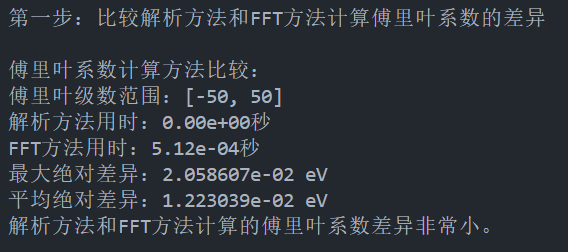
\includegraphics[width=1.0\textwidth]{Problem_1/figs/1_vq_coeff.png}
    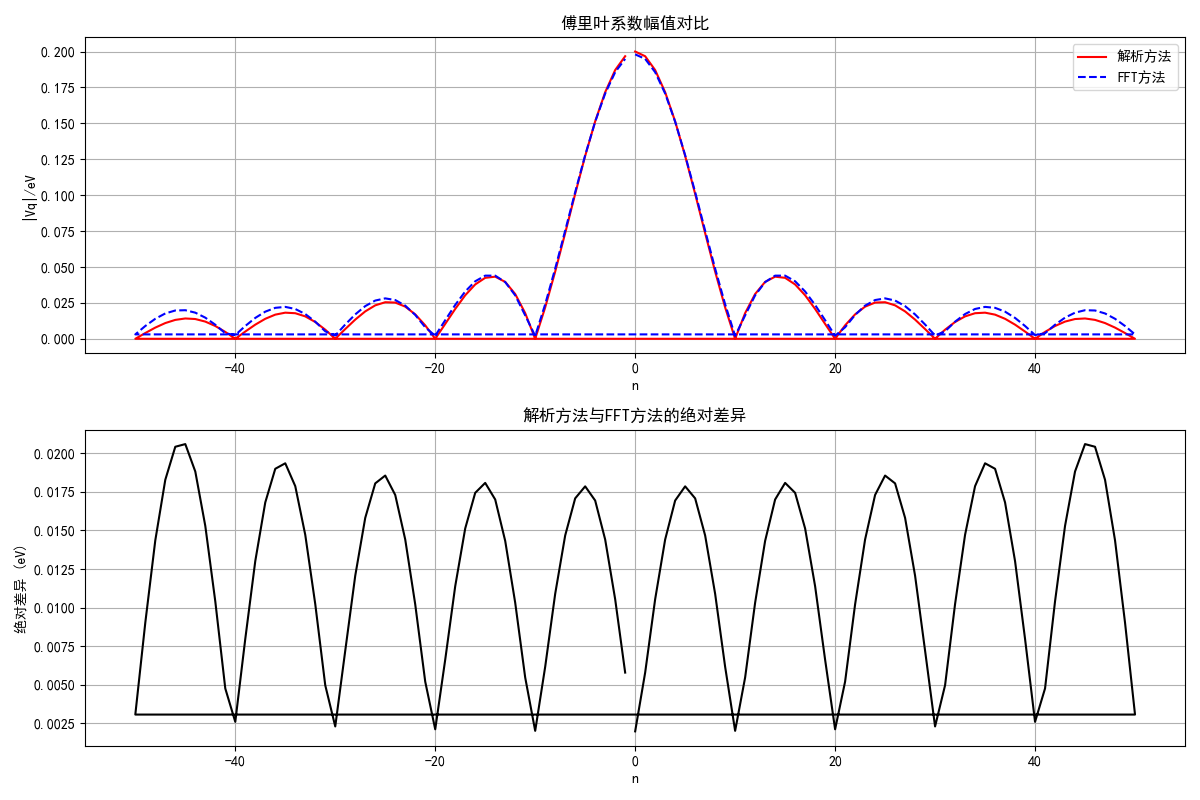
\includegraphics[width=1.0\textwidth]{Problem_1/figs/vq_coeff.png}
    \caption{第一步:比较解析计算与FFT得到的势能傅里叶系数}
\end{figure}

\begin{figure}[H]
    \centering
    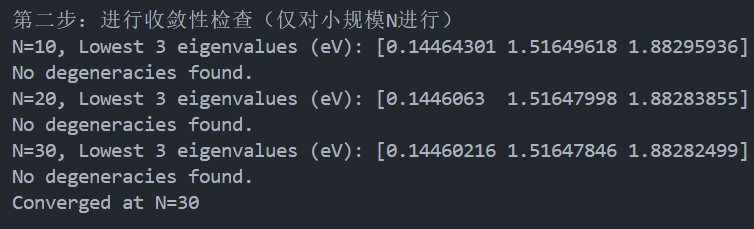
\includegraphics[width=1.0\textwidth]{Problem_1/figs/2_converge.png}
    \caption{第二步:收敛性检查}
\end{figure}

\begin{figure}[H]
    \centering
    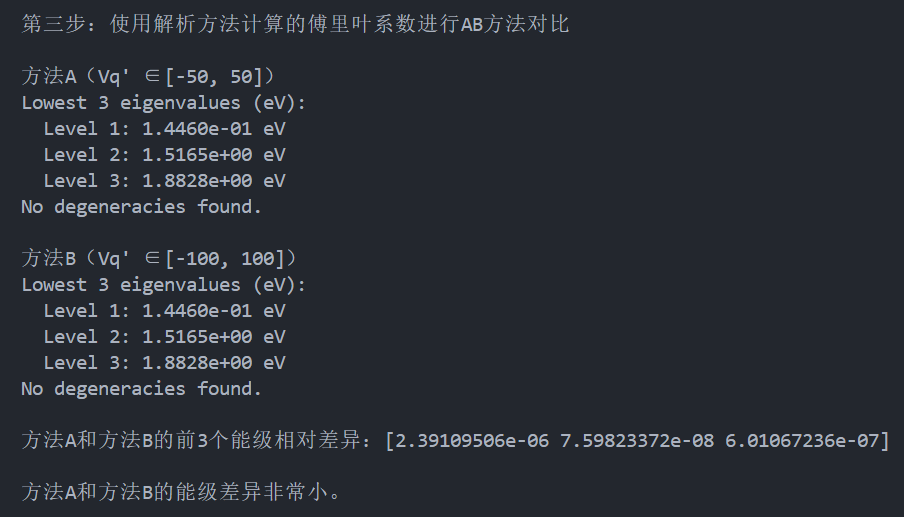
\includegraphics[width=1.0\textwidth]{Problem_1/figs/3_comparison.png}
    \caption{第三步:不同势能展开范围的AB方法对比}
\end{figure}

\begin{figure}[H]
    \centering
    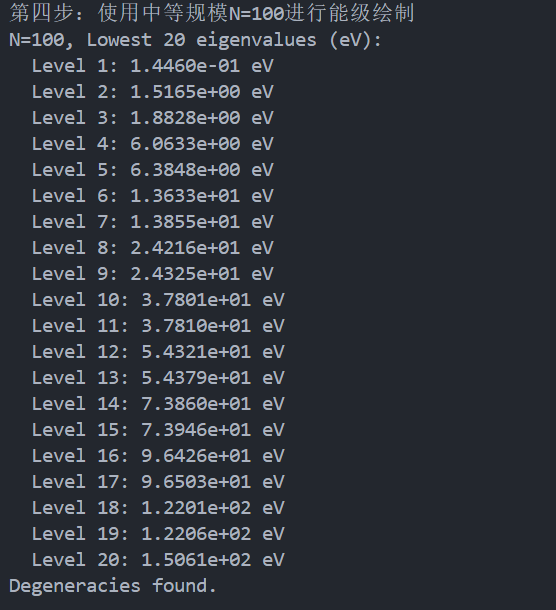
\includegraphics[width=0.55\textwidth]{Problem_1/figs/4_medium.png}
    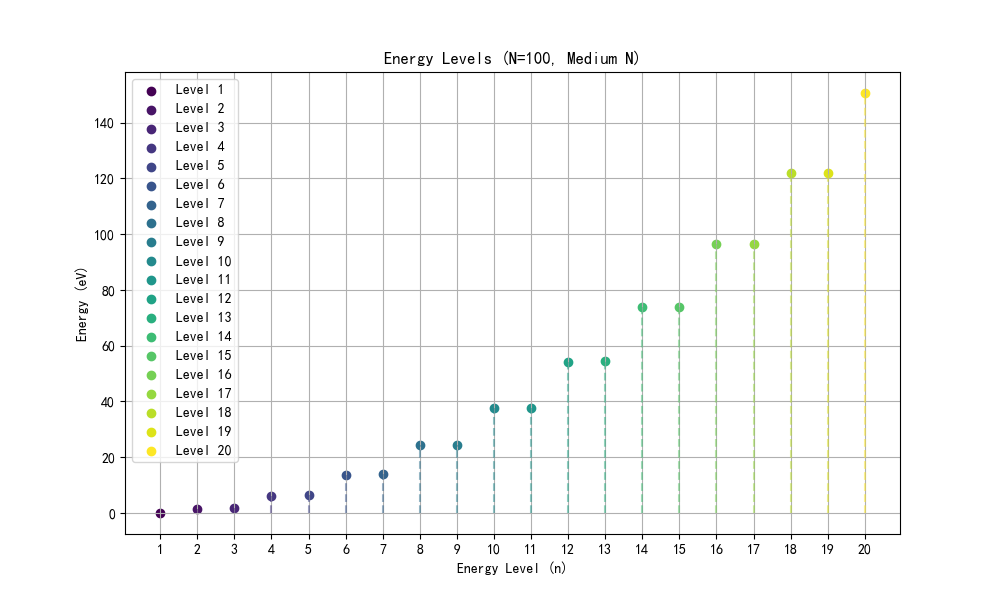
\includegraphics[width=0.5\textwidth]{Problem_1/figs/energy_levs_medium.png}
    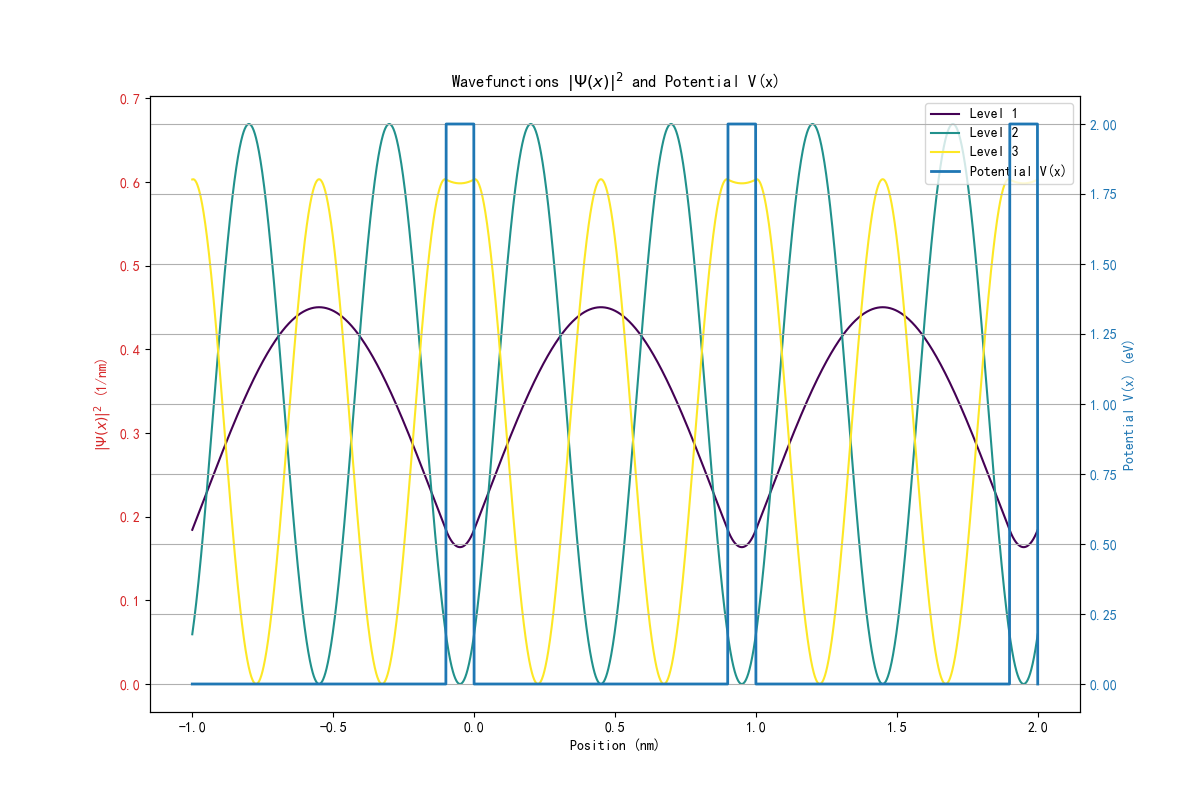
\includegraphics[width=0.5\textwidth]{Problem_1/figs/wave_funcs.png}
    \caption{第四步:进行中等规模$N=100,num\_levels=20$的计算与绘制,并绘制势阱与前三个能级的波函数}
\end{figure}

\begin{figure}[H]
    \centering
    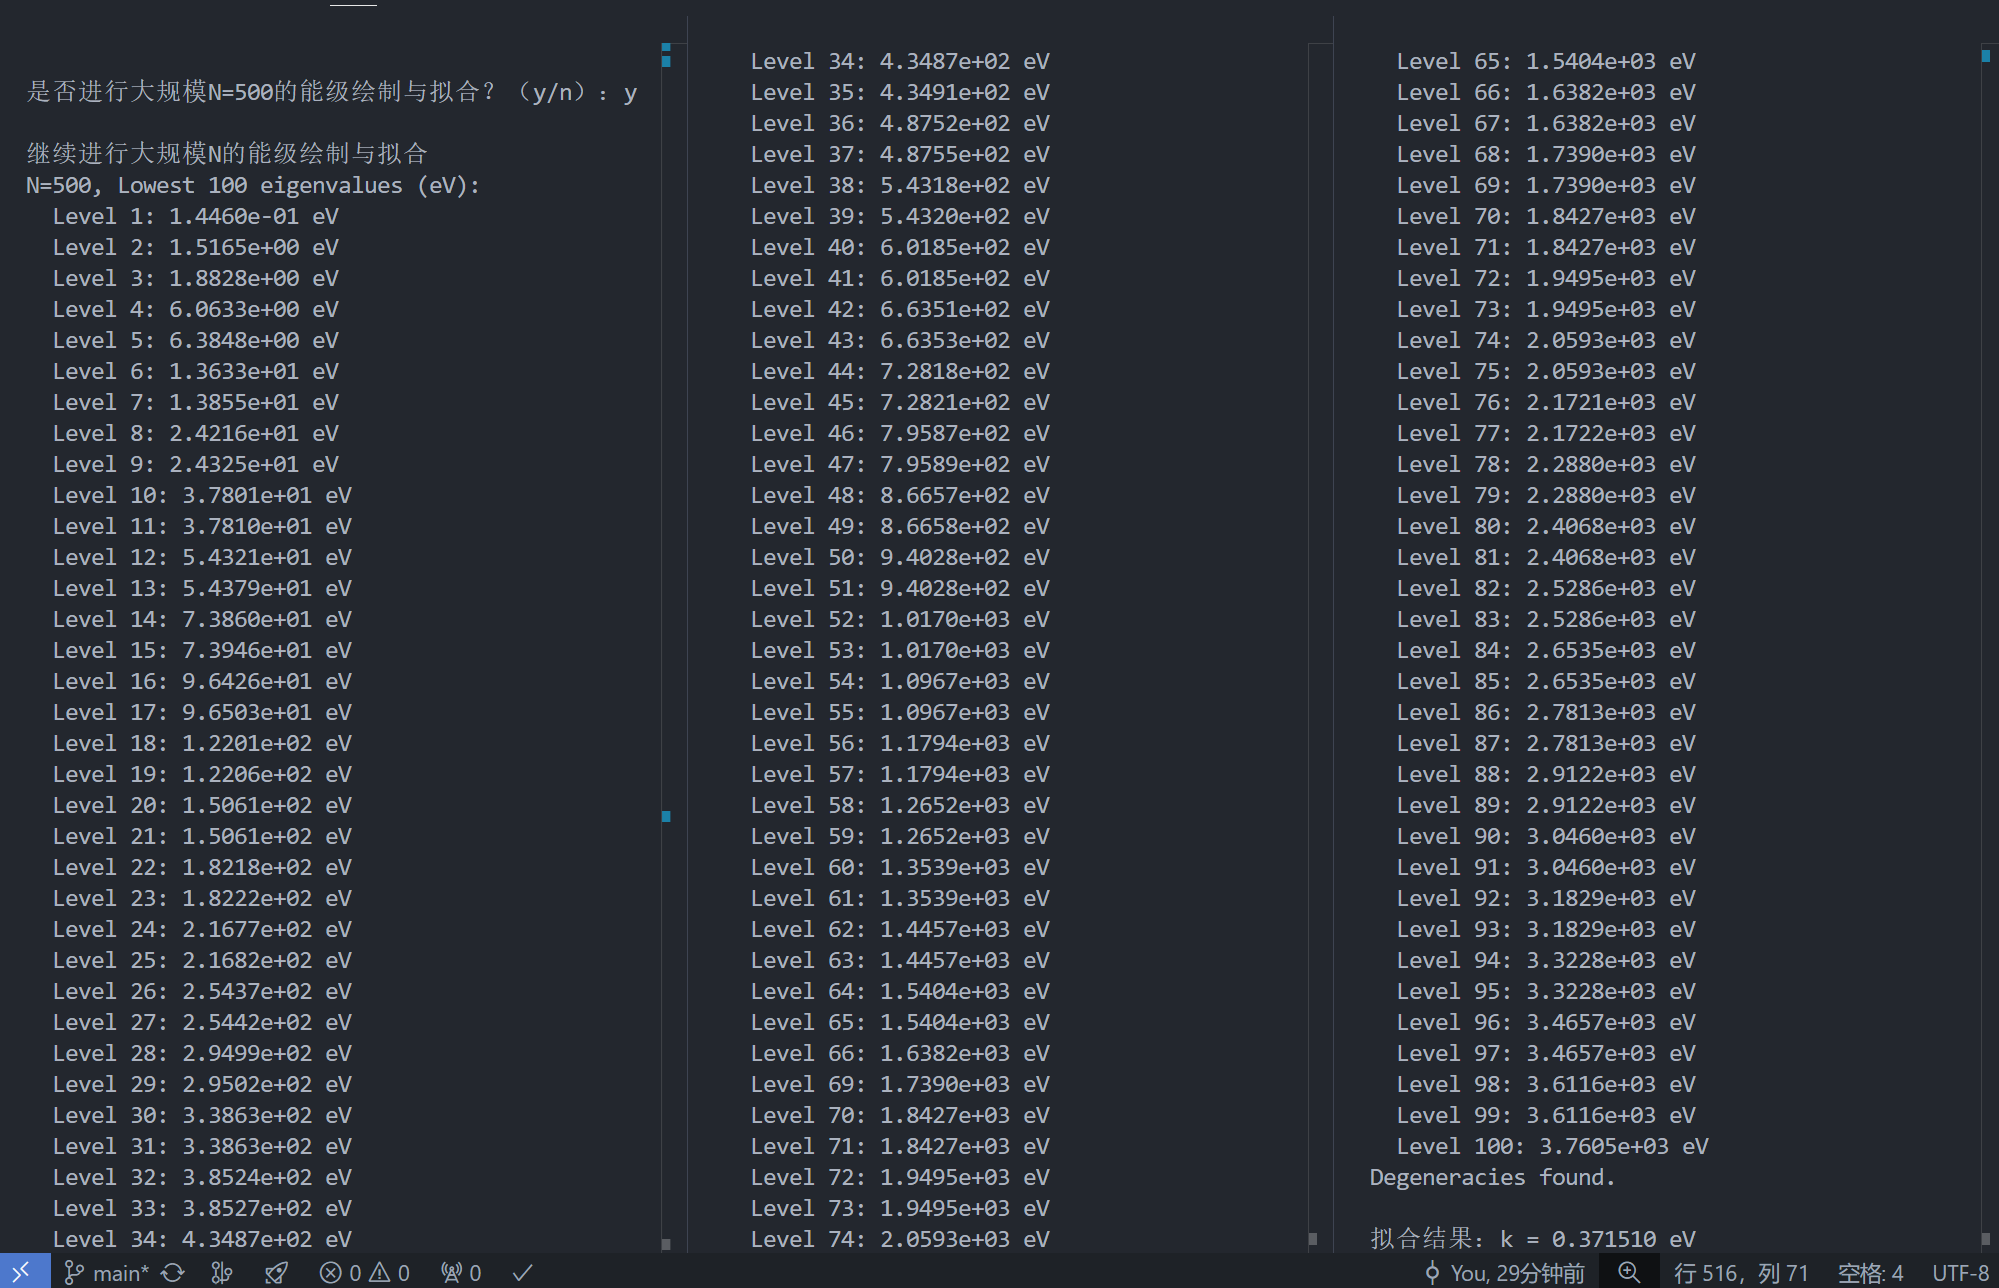
\includegraphics[width=1.0\textwidth]{Problem_1/figs/5_large.png}
    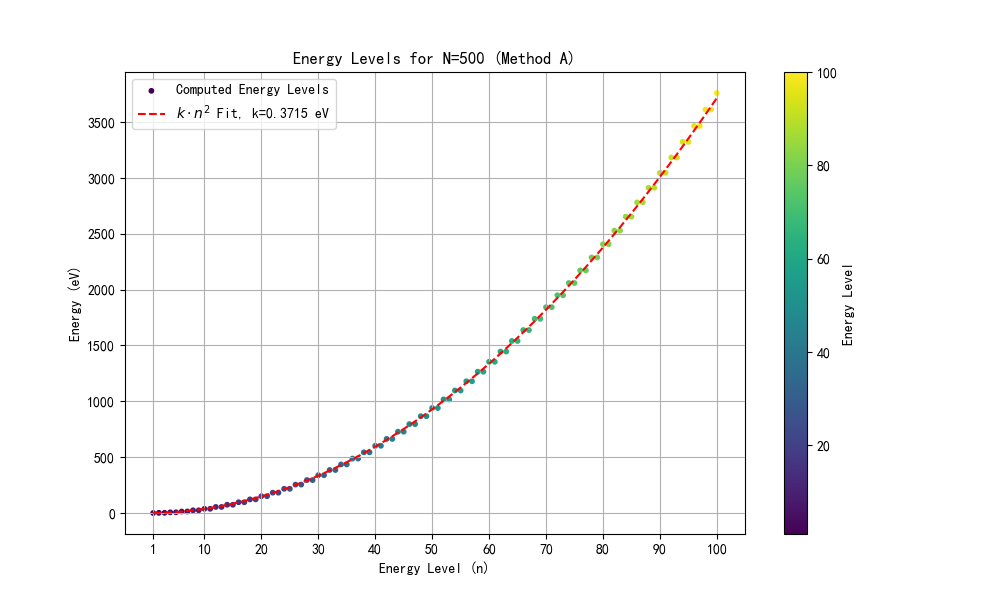
\includegraphics[width=1.0\textwidth]{Problem_1/figs/energy_levs_large.png}
    \caption{第五步:进行大规模$N=500,num\_levels=100$的计算与绘制,并进行拟合}
\end{figure}

